\chapter{Introduzione}  
La stima della profondità ha da sempre rappresentato un problema di massimo interesse. L'informazione sulla profondità è importante, ed in alcuni casi essenziale, per molteplici applicazioni pratiche della visione artificiale: guida autonoma, robotica, ricostruzione 3D e realtà aumentata sono soltanto alcune. \\
L'acquisizione delle geometrie tridimensionali di scene del mondo reale rappresenta da sempre un problema complesso, e gli strumenti sono stati accessibili soltanto in grosse compagnie e centri di ricerca. Nel corso degli anni, molte tecniche sono state sviluppate e nuovi dispositivi, dai costi più ridotti, sono stati introdotti nel mercato.\\
Le principali tecnologie per la percezione dell'ambiente sfruttano sensori ottici che catturano la luce visibile o infrarossa che viene riflessa dalla scena. Questo lavoro di tesi tratta due categorie di sensori in particolare, entrambi molto diffusi e accessibili: i sensori a visione stereoscopica e i sensori basati sul tempo di volo (Time-Of-Flight, ToF).\\
Nello stesso periodo, nel mondo della computer vision, il machine learning (e deep learning in particolare) si è dimostrato uno strumento che ha ampiamente incrementato le prestazioni rispetto ad altri metodi deterministici, in molti problemi ritenuti complessi, fino a superare le prestazioni umane. E proprio grazie al machine learning è stato possibile sviluppare sistemi efficaci per la ricostruzione delle informazioni catturate dai sensori.

\section{Descrizione del progetto}
L'obiettivo del lavoro di questa tesi è lo sviluppo di un sistema di machine learning per la fusione dei dati tridimensionali forniti dai sensori, cercando di fornire una ricostruzione più accurata. La scelta dei sensori gioca perciò un ruolo fondamentale: le telecamere stereo e il sensore ToF tendono ad avere caratteristiche complementari, e la loro combinazione si è rivelato efficace negli ultimi anni. 

\section{Principi di funzionamento del sistema di acquisizione}
Il sistema di acquisizione è composto da una coppia di telecamere stereo e da un sensore Time-of-Flight disposti adiacentemente. I due dispositivi catturano la stessa scena allo stesso istante.

\begin{figure}[ht]
    \centering
    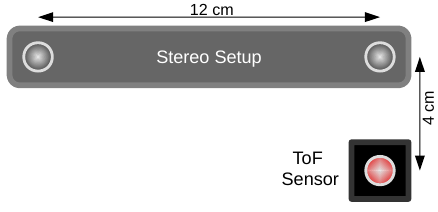
\includegraphics[width=0.5\columnwidth]{tof_stereo_acquisition_system}
    \caption[Sistema di acquisizione ToF-Stereo]{Rappresentazione del sistema di acquisizione ToF-Stereo. Il sensore ToF è posizionato sotto la telecamera di riferimento della coppia stereo.}
    \label{etichetta}
\end{figure}

\subsection{Sistema di visione stereo}
Il sensore a visione stereoscopica consiste nell'acquisire due immagini bidimensionali da una coppia di telecamere rettificate, ossia allineate lungo un asse che inquadrano la stessa scena. Lo stesso punto P dello spazio viene proiettato nel piano dell'immagine di ciascuna delle telecamere. I punti risultanti \(p_L\) e \(p_R\), detti \textit{omologhi}, hanno le stesse coordinate verticali, considerata la rettificazione dei sensori. Viene chiamata \textit{disparità} lo scostamento tra le coordinate orizzontali: \[d = u_L - u_R\] Tramite questo valore è possibile determinare la posizione del punto P nello spazio.\\
Uno dei principali vantaggi è il costo ridotto delle telecamere CCD o CMOS, facilmente accessibili nel mercato. Tale sensore è inoltre passivo, quindi può sfruttare l’illuminazione dell’ambiente. Ciò permette di essere utilizzato in ambienti esterni, al contrario di altri sensori che sfruttano
pattern proiettati con illuminatori. Inoltre può avere alte risoluzioni e una limitata quantità di rumore.\\
Lo svantaggio maggiore è la dipendenza dei risultati forniti da questi sensori dalla tessitura delle immagini utilizzata nel calcolo degli omologhi, ad esempio uno sfondo uniforme o ripetitivo è difficilmente individuabile. Pertanto essi presentano un’accuratezza solitamente limitata.

\subsection{Sensore Time-Of-Flight}

\section{Il Machine learning}

\subsection{Reti neurali artificiali}

\subsection{Reti neurali convoluzionali}